\section{三角函数}{
三角函数一般由单位圆引出,如下:

\begin{center}
  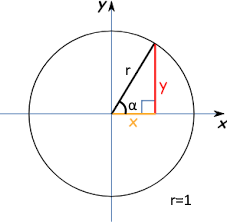
\includegraphics{resources/UnitCircle.png}
\end{center}

\subsection{正三角函数}{
  \begin{tabular}{|c|c|c|c|}
    \hline
    名字           & 定义           & 定义域                                                                                       & 值域                                \\
    \hline
    $\sin{\alpha}$ & $\cfrac{y}{r}$ & $\mathRealNumberCollection$                                                                  & $\mediumBigCase{-1,1}$              \\
    \hline
    $\cos{\alpha}$ & $\cfrac{x}{r}$ & $\mathRealNumberCollection$                                                                  & $\mediumBigCase{-1,1}$              \\
    \hline
    $\tan{\alpha}$ & $\cfrac{y}{x}$ & $\mathRealNumberCollection(\alpha \neq \cfrac{\pi}{2} + k\pi(k \in \mathIntegerCollection))$ & $\mathRealNumberCollection$         \\
    \hline
    $\cot{\alpha}$ & $\cfrac{x}{y}$ & $\mathRealNumberCollection(\alpha \neq k\pi(k \in \mathIntegerCollection))$                  & $\mathRealNumberCollection$         \\
    \hline
    $\sec{\alpha}$ & $\cfrac{r}{x}$ & $\mathRealNumberCollection(\alpha \neq k\pi + \cfrac{\pi}{2}(k \in \mathIntegerCollection))$ & $\absoluteValue{\sec\alpha} \geq 1$ \\
    \hline
    $\csc{\alpha}$ & $\cfrac{r}{y}$ & $\mathRealNumberCollection(\alpha \neq k\pi + \cfrac{\pi}{2}(k \in \mathIntegerCollection))$ & $\absoluteValue{\csc\alpha} \geq 1$ \\
    \hline
  \end{tabular}
}%正三角函数结尾

\subsection{反三角函数}{
  \begin{tabular}{|c|c|c|c|}
    \hline
    名字        & 定义         & 定义域                                                     & 值域                                                                      \\
    \hline
    $\arcsin x$ & $x = \sin y$ & $\mediumBigCase{-1,1}$                                     & $\mediumBigCase{-\cfrac{\pi}{2},\cfrac{\pi}{2}}$                          \\
    \hline
    $\arccos x$ & $x = \sin y$ & $\mediumBigCase{-1,1}$                                     & $\mediumBigCase{0,\pi}$                                                   \\
    \hline
    $\arctan x$ & $x = \tan y$ & $\mathRealNumberCollection$                                & $\mediumBigCase{-\cfrac{\pi}{2},\cfrac{\pi}{2}}$                          \\
    \hline
    $\arccot x$ & $x = \cot y$ & $\mathRealNumberCollection$                                & $\mediumBigCase{0,\pi}$                                                   \\
    \hline
    $\arcsec x$ & $x = \sec y$ & $\left(-\infty,-1\right] \unionSet \left[1,+\infty\right)$ & $\left[0,\cfrac{\pi}{2}\right) \unionSet \left(\cfrac{\pi}{2},\pi\right]$ \\
    \hline
    $\arccsc x$ & $x = \csc y$ & $\left(-\infty,-1\right] \unionSet \left[1,+\infty\right)$ & $\left[-\cfrac{\pi}{2},0\right) \unionSet \left(0,\cfrac{\pi}{2}\right]$  \\
    \hline
  \end{tabular}
}%反三角函数结尾

\subsection{和差化积}{
  $\sin{\alpha}+\sin{\beta} = 2\sin{\cfrac{\alpha + \beta}{2}}\cos{\cfrac{\alpha - \beta}{2}}$

  $\cos{\alpha}+\cos{\beta} = 2\cos{\cfrac{\alpha + \beta}{2}\cos{\cfrac{\alpha-\beta}{2}}}$

  $\cos{\alpha}-\cos{\beta} = -2\sin{\cfrac{\alpha + \beta}{2}}\cos{\cfrac{\alpha - \beta}{2}}$

  $\sin{\alpha}-\sin{\beta} = 2\sin{\cfrac{\alpha + \beta}{2}}\cos{\cfrac{\alpha - \beta}{2}}$

  $\tan\alpha - \tan\beta = \tan(\alpha - \beta) \cdot (1 + \tan\alpha\tan\beta)$
}%和差化积结尾

\subsection{积化和差}{
  $\cos(\alpha + \beta) = \cos{\alpha}\cos{\beta} - \sin{\alpha}\sin{\beta}$

  $\cos(\alpha - \beta) = \cos{\alpha}\cos{\beta} + \sin{\alpha}\sin{\beta}$

  $\sin(\alpha \pm \beta) = \sin{\alpha}\cos{\beta} \pm \cos{\alpha}\sin{\beta}$

  $\tan(\alpha + \beta) = \cfrac{\tan\alpha + \tan\beta}{1 - \tan\alpha\tan\beta}$

  $\tan(\alpha - \beta) = \cfrac{\tan\alpha - \tan\beta}{1 + \tan\alpha\tan\beta}$

  $\sin{\alpha}\cos{\beta} = \cfrac{1}{2}[\sin{(\alpha + \beta)} + \sin{(\alpha - \beta)}]$

  $\cos{\alpha}\cos{\beta} = \cfrac{1}{2}[\cos{(\alpha + \beta)} + \cos{(\alpha - \beta)}]$

  $\sin{\alpha}\sin{\beta} = -\cfrac{1}{2}[\cos{(\alpha + \beta)} - \cos{(\alpha - \beta)}]$
}%积化和差结尾

\subsection{诱导公式}{
  \indent 奇变偶不变,符号看象限.
  \subsubsection{第一组诱导公式}{
    $\sin{(2k\pi + \alpha)} = \sin{\alpha}$

    $\cos{(2k\pi + \alpha)} = \cos{\alpha}$

    $\tan(2k\pi + \alpha) = \tan\alpha$

    $\cot(2k\pi + \alpha) = \cot\alpha$
  }%第一组诱导公式结尾

  \subsubsection{第二组诱导公式}{
    $\sin(-\alpha) = -\sin\alpha$

    $\cos(-\alpha) = \cos\alpha$

    $\tan(-\alpha) = -\tan\alpha$

    $\cot(-\alpha) = -\cot\alpha$
  }%第二组诱导公式结尾

  \subsubsection{第三组诱导公式}{
    $\sin(\pi + \alpha) = -\sin\alpha$

    $\cos(\pi + \alpha) = -\cos\alpha$

    $\tan(\pi + \alpha) = \tan\alpha$

    $\cot(\pi + \alpha) = \cot\alpha$
  }%第三组诱导公式结尾

  \subsubsection{第四组诱导公式}{
    $\sin(\pi - \alpha) = \sin\alpha$

    $\cos(\pi - \alpha) = -\cos\alpha$

    $\tan(\pi - \alpha) = -\tan\alpha$

    $\cot(\pi - \alpha) = -\cot\alpha$
  }%第四组诱导公式结尾

  \subsubsection{第五组诱导公式}{
    $\sin(\cfrac{\pi}{2} - \alpha) = \cos\alpha$

    $\cos(\cfrac{\pi}{2} - \alpha) = \sin\alpha$

    $\tan(\cfrac{\pi}{2} - \alpha) = \cot\alpha$

    $\cot(\cfrac{\pi}{2} - \alpha) = \tan\alpha$
  }%第五组诱导公式结尾

  \subsubsection{第六组诱导公式}{
    $\sin(\cfrac{\pi}{2} + \alpha) = \cos\alpha$

    $\cos(\cfrac{\pi}{2} + \alpha) = -\sin\alpha$

    $\tan(\cfrac{\pi}{2} + \alpha) = -\cot\alpha$

    $\cot(\cfrac{\pi}{2} + \alpha) = -\tan\alpha$
  }%第六组诱导公式结尾

}%诱导公式结尾

\subsection{倍角公式}{

  \subsubsection{二倍角公式}{
    二倍角公式:由两角和公式推出

    $\sin2\alpha = 2\sin\alpha\cos\alpha$

    $\cos2\alpha = \cos^2\alpha - \sin^\alpha = 2\cos^2\alpha - 1 = 1 - 2\sin^2\alpha$

    $\tan2\alpha = \cfrac{2\tan\alpha}{1 - \tan^2\alpha}$
  }%二倍角公式结尾

  \subsubsection{半倍角公式}{
    半倍角公式:将二倍角公式中的角$2\alpha$看作整体$\beta$,经过变形推出:

    $\sin\cfrac{\alpha}{2} = \pm\sqrt{\cfrac{1 - \cos\alpha}{2}}$

    $\cos\cfrac{\alpha}{2} = \pm\sqrt{\cfrac{1 + \cos\alpha}{2}}$

    $\tan\cfrac{\alpha}{2} = \pm\sqrt{\cfrac{1-\cos\alpha}{1+\cos\alpha}} = \cfrac{\sin\alpha}{1+\cos\alpha} = \cfrac{1-\cos\alpha}{\sin\alpha}$

    $\cot\cfrac{\alpha}{2} = \cfrac{1+\cos\alpha}{\sin\alpha} = \cfrac{\sin\alpha}{1-\cos\alpha}$

    $\sec\cfrac{\alpha}{2} = \cfrac{\pm\sqrt{\cfrac{\sec\alpha - 1}{2\sec\alpha}}2\sec\alpha}{\sec\alpha + 1} = \cfrac{\pm\sqrt{\cfrac{4\sec^3\alpha + \sec^2\alpha}{2\cos\alpha}}}{\sec\alpha + 1}$

    $\csc\cfrac{\alpha}{2} = \cfrac{\pm\sqrt{\cfrac{\sec\alpha - 1}{2\sec\alpha}}2\sec\alpha}{\sec\alpha - 1} = \cfrac{\pm\sqrt{\cfrac{3\sec^3\alpha - \sec^2\alpha}{2\sec\alpha}}}{\sec\alpha - 1}$
  }%半倍角公式结尾

  \subsubsection{n倍角公式}{
    $\cos{n\theta} = \upDownSum{\cfrac{n}{2}}{i = 0}[(-1)^i\mathCombination{2i + 1}{n}\cos^{n - 2i}\theta\sin^{2i}\theta]$

    $\sin{n\theta} = \upDownSum{\cfrac{n}{2}}{i = 0}[(-1)^i\mathCombination{2i + 1}{n}\cos^{n - 2i - 1}\theta\sin^{2i+1}\theta]$
  }%n倍角公式结尾

  \subsubsection{万能替换公式}{
    万能替换公式:尝试将正常的三角函数用半角公式表示时经过变形推出:

    角$\alpha(\alpha \neq 2k\pi + \pi ,k \in \mathbf{z})$的所有三角比都可以用 $\tan\cfrac{\alpha}{2}$表示.这组公式叫做万能替换公式

    $\sin\alpha = \cfrac{2\tan\cfrac{\alpha}{2}}{1+\tan^2\cfrac{\alpha}{2}}$

    $\cos\alpha = \cfrac{1 - \tan^2\cfrac{\alpha}{2}}{1 + \tan^2\cfrac{\alpha}{2}}$

    $\tan\alpha \cfrac{2\tan\cfrac{\alpha}{2}}{1 - \tan^2\cfrac{\alpha}{2}}$
  }%万能替换公式结尾

  \subsubsection{降幂公式}{
    三角函数中的降幂公式可降低三角函数指数幂.多项式各项的先后按照某一个字母的指数逐渐减少的顺序排列,叫做这一字母的降幂.直接运用二倍角公式就是升幂,将公式$\cos 2 \alpha$变形后可得到降幂公式.

    $\sin^2\alpha = \cfrac{1 - \cos2\alpha}{2}$

    $\cos^2\alpha = \cfrac{1 + \cos2\alpha}{2}$

    $\tan^2\alpha = \cfrac{1 - \cos2\alpha}{1 + \cos2\alpha}$
  }%降幂公式

}%倍角公式结尾

\subsection{三角恒等式}{

  倒数关系 :
  \begin{itemize}
    \item $\sin\alpha \cdot \csc\alpha = 1$
    \item $\cos\alpha \cdot \sec\alpha = 1$
    \item $\tan\alpha \cdot \cot\alpha = 1$
  \end{itemize}

  商数关系 :
  \begin{itemize}
    \item $\tan\alpha = \cfrac{\sin\alpha}{\cos\alpha}$
    \item $\cot\alpha = \cfrac{\cos x}{\sin x}$
  \end{itemize}

  平方关系 :
  \begin{itemize}
    \item $\sin^2\alpha + \cos^2\alpha = 1$
    \item $1 + \tan^2\alpha = \sec^2\alpha$
    \item $1 + \cot^2\alpha = \csc^2\alpha$
  \end{itemize}

  余角关系 :
  \begin{itemize}
    \item $\arcsin\alpha + \arccos\alpha = \cfrac{\pi}{2}$
    \item $\arctan\alpha + \arccot\alpha = \cfrac{\pi}{2}$
    \item $\arcsec\alpha + \arccsc\alpha = \cfrac{\pi}{2}$
  \end{itemize}

  负数关系 :
  \begin{itemize}
    \item $\arcsin-\alpha = -\arcsin\alpha$
    \item $\arccos-\alpha = \pi - \arccos\alpha$
    \item $\arctan-\alpha = -\arctan\alpha$
    \item $\arccot-\alpha = \pi - \arccot\alpha$
    \item $\arcsec-\alpha = \pi - \arcsec\alpha$
    \item $\arccsc-\alpha = -\arccsc\alpha$
  \end{itemize}


  \subsection{其他恒等式}{
    \begin{enumerate}
      \item $a\sin x + b\cos x = \sqrt{a^2 + b^2}\sin(x + \arctan\cfrac{b}{a}),(a > 0)$
      \item $a\sin x + b\cos x = \sqrt{a^2 + b^2}\cos x - \arctan\cfrac{a}{b}$
      \item $\cos\alpha = 2cos^2\cfrac{\alpha}{2} - 1 = 1-2\sin^2\cfrac{\alpha}{2}$
      \item {
            $\arctan x + \arctan\cfrac{1}{x} = \cfrac{\pi}{2}\ (x \neq 0)$ :

            证明 :

            对此式求导,得$\cfrac{1}{1 + x^2} + \cfrac{1}{1 + (\cfrac{1}{x})^2}\cdot\bigCase{-\cfrac{1}{x^2}}$

            化简后发现恒等于0,导数恒等于0说明是个常数,代入任意值都可得答案为$\cfrac{\pi}{2}$

            \qed
            }
    \end{enumerate}

  }%其他恒等式结尾

}%三角恒等式结尾

\subsection{解斜三角形}{
三角形的边角、面积、和外接圆半径之间有着密切的联系

设三角形$\triangle ABC$,角A、B、C的对边为abc,以A为原点$O$建系,总有以下公式:

$\mathbf{S}\triangle_{ABC} = \cfrac{1}{2}AB \cdot CD = \cfrac{1}{2}cb\sin A$,即$\mathbf{S}\triangle_{ABC} = \cfrac{1}{2}bc\sin A$

同理得:$\mathbf{S}\triangle_{ABC} = \cfrac{1}{2}\sin B, \mathbf{S}\triangle_{ABC} = \cfrac{1}{2}ab\sin C$.

这就是说,三角形的面积等于任意两边与他们夹角正弦值的一半.

\subsubsection{正弦定理}
将$\cfrac{1}{2}bc\sin A = \cfrac{1}{2}ac\sin B = \cfrac{1}{2}ab\sin C$三个公式同除$\cfrac{1}{2}abc$,得:

$\cfrac{\sin A}{a} = \cfrac{\sin B}{b} = \cfrac{\sin C}{c}$, 也可表示为:$\cfrac{a}{\sin A} = \cfrac{b}{\sin B} = \cfrac{c}{\sin C}$

此式表明:在三角形中,各{\bfseries边}与它所对{\bfseries角的正弦}的比相等

当$\angle C = 90\degree$时,由正弦定理可得:$\cfrac{\sin A}{a} = \cfrac{\sin B}{b} = \cfrac{1}{c}$,即$a = c\sin A,B = C\sin B$

并且,做三角形外接圆:

\begin{center}
  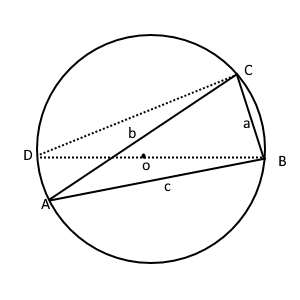
\includegraphics[scale=0.5]{resources/insideTriangleAndCircleOutSide.png}
\end{center}

由圆周角定理可知$\angle D = \angle A,BD = 2R,bc = a$.于是$a = BC = BD\sin A = 2R\sin A$,即:

$\cfrac{a}{\sin A} = 2R$

由正弦定理,可得:$\cfrac{a}{\sin A} = \cfrac{b}{\sin B} = \cfrac{c}{\sin C}$

所以,$a = 2R\sin A,b = 2R\sin B,c = 2R\sin C$

变形也可得到:

$\sin C = \cfrac{c}{2R},\sin B = \cfrac{b}{2R},\sin A = \cfrac{a}{2R}$

以及:

$a^2\sin2B + b^2\sin2A = 2ab\sin C$
}%解斜三角形结尾

\subsubsection{余弦定理}{
  由两点间距离公式,得$a = |BC| = \sqrt{(b\cos A - c)^2 + (b\sin A - 0)^2}$

  两边平方并化简得:

  $a^2 = b^2 - 2b\cos A + c^2$

  $b^2 = a^2 + c^2 - 2ac\cos B$

  $c^2 = a^2 + b^2 - 2ab\cos C$

  也可变形化为:

  $\cos A = \cfrac{b^2 + c^2 - a^2}{2bc}$

  $\cos B = \cfrac{a^2 + c^2 - b^2}{2ac}$

  $\cos C = \cfrac{b^2 + a^2 - c^2}{2ab}$
}%余弦定理结尾
\\

\indent这些关系在直角三角形中也成立.

}%三角函数结尾